\chapter{面向异构后端的容器内存压力感知卸载架构设计与实现}

本章详细介绍了面向容器环境的异构分层内存协同卸载系统的设计与实现细节。该系统采用了一种新颖的内核态-用户态协同方法,以实现对内存压力的精确感知和对容器工作集的动态优化。本研究将内存压力定义为由于内存资源不足而导致的应用程序性能下降,具体表现为同步内存回收操作所占用的时间片比例。基于此,我们首先在内核层构建了一个细粒度的内存压力模型,该模型能够实时、准确地反映系统的内存受限程度;基于该模型,我们在用户态设计了一种自适应的工作集估计算法,该算法能够根据内存压力动态调整容器的内存资源分配。为了清晰地阐述系统的各个方面,本章将依次介绍系统的整体架构、内核态的内存压力建模与监控机制、用户态的自适应工作集估算与 cgroup 集成,并通过架构图、流程图、伪代码和具体实例对关键技术进行详细说明。

\section{系统架构总览}

为实现容器化应用在异构分层内存环境下的高效卸载,本系统构建了一个内核态与用户态紧密协同的负反馈调节系统。该系统以内存压力作为核心驱动信号,动态、精细化地调整容器工作集,构成一个自适应的闭环控制回路。相比传统基于缺页中断、内存分配次数等统计信息进行工作集估算的方法,本系统能够更灵敏地感知内存资源紧张程度,更准确地预测内存需求变化,从而避免内存过度分配或不足,保证应用程序的服务质量,并提升整体资源利用效率。

\begin{figure}[h]
    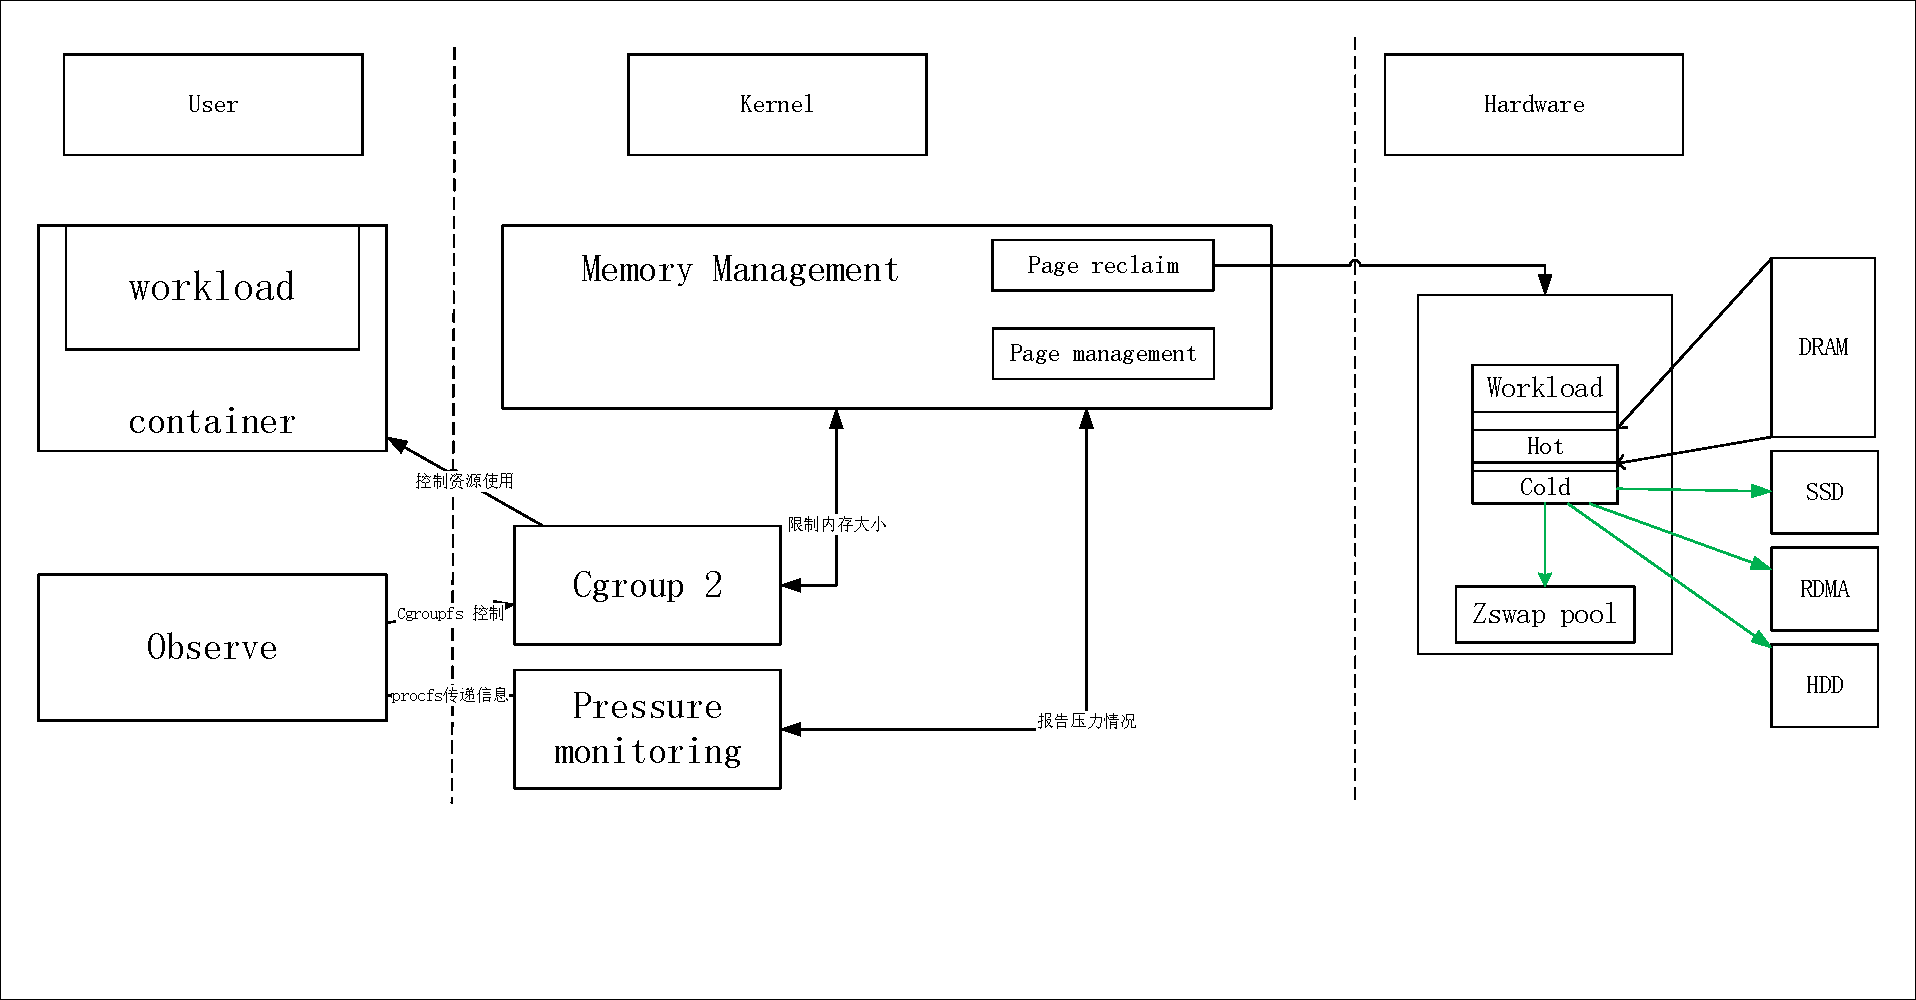
\includegraphics[width=\textwidth, keepaspectratio]{架构图设计.pdf}
    \caption{架构图设计}
    \label{架构图设计}
\end{figure}

如图 \ref{架构图设计} 所示,本系统采用层次化设计,横跨用户空间、内核空间以及硬件层。在容器内部,运行着用户的工作负载,其产生的内存访问请求由内核的内存管理子系统进行处理。

用户空间部署了两个关键组件:工作集估算器(Working Set Estimator, WSE)和 cgroup 管理器。WSE 扮演着感知、决策和执行的角色,它通过 /proc 文件系统等机制持续地从内核态的内存压力监控器获取实时的内存压力信息。不同于传统的周期性轮询,WSE 还支持基于事件的通知机制,以实现更及时的响应。

内核空间的核心组件是内存压力监控器(Pressure Monitoring, PM)。PM 并非简单的统计模块,而是一个深度嵌入到内核内存管理子系统中的主动监控与分析单元,它与内存分配、页面回收等关键路径紧密集成。具体而言,PM 采用类似于静态插桩的技术,在每次发生同步内存回收时,记录本次同步中断所占用的时间片,并与调度系统交互以计算回收延迟,生成一个量化的压力信号(例如,数值或等级),该信号通过 /proc 文件系统周期性地暴露给用户空间。此外,为了减少用户空间轮询的开销,PM 还实现了基于事件的通知机制,当内存压力超过预设阈值时,主动通知用户空间的工作集估算器。

本系统的核心在于其负反馈调节机制,该机制通过内核态与用户态的紧密协同,实现对容器内存资源的动态、精细化管理。内核态的PM持续监测系统的内存使用状况,并生成量化的压力信号。该信号通过 /proc 文件系统等机制周期性地暴露给用户空间,同时支持基于事件的通知机制,以便在压力变化时及时通知用户空间的WSE。当系统内存压力较低时,表明内存资源相对充裕。此时,WSE 会指示 cgroup 管理器收缩容器的内存分配上限。这一操作的目的在于主动触发内核的页面回收机制。由于容器的内存使用受到更严格的限制,内核会更积极地回收不活跃的冷页面,将它们换出到分层存储上。这种策略的核心思想是"预先释放,主动应对",避免了在内存压力突然增大时才被动地进行页面回收,从而减少了应用程序因内存回收而产生的延迟。当系统整体内存压力升高时(例如,由于其他容器的内存需求增加),PM 会迅速检测到这一变化,并更新其输出的压力信号(例如,提高压力等级或触发事件通知)。WSE 接收到升高的压力信号后,会触发负反馈调节。它会重新评估当前容器的内存需求,并根据预定义的策略(这些策略会综合考虑容器的优先级、历史内存使用情况、服务质量要求等因素,并将在后续章节详细阐述)计算出一个更大的工作集大小。随后,WSE 通过与 cgroup 管理器的交互,将新的工作集大小转化为对 cgroup v2 内存限制参数的具体设置。cgroup 管理器通过调整 cgroup v2 提供的接口(例如 memory.high, memory.max 等),放宽对容器内存使用量的限制,允许容器保留更大的工作集。这样做可以减少因内存不足而导致的缺页中断,从而保障应用程序的性能。

上述过程形成了一个完整的负反馈闭环:内核态的 PM 提供实时的压力反馈(作为反馈信号),用户态的 WSE 根据压力信号进行决策(作为控制器),cgroup 管理器执行资源控制(作为执行器),容器的工作负载在调整后的资源约束下运行(作为被控对象)。容器的内存访问行为会进一步影响内核的内存压力,从而形成一个持续的、自适应的动态调节循环。这种内核态与用户态紧密协同的负反馈机制,使得系统能够灵敏、准确地响应内存压力的变化,在保证关键应用性能的同时,最大化异构内存系统的整体利用率,并有效避免了因内存过度分配导致的系统抖动和性能下降。此外,由于采用了更细粒度的压力信号和更及时的响应机制,本系统相比传统的基于粗粒度统计信息(如缺页中断次数)的方案,具有更高的稳定性和鲁棒性。


\section{基于同步回收延迟的内存压力量化算法的设计与实现}

这一章的核心目标是详细阐述基于同步回收延迟的内存压力量化算法的设计思想、具体实现步骤、以及实现中的关键技术细节。

\subsection{同步回收延迟与内存压力的关联分析}

在传统的内存管理研究中,工作集估计算法扮演着重要角色,其准确性直接影响着内存分配、页面置换等关键决策。鉴于工作集估计算法高度依赖于对系统内存压力的准确量化,本节首先深入剖析同步回收延迟与内存压力之间的内在关联。

传统的工作集估计算法,如WSE (Working Set Estimation) 和WSE-Lite,通常依赖于对缺页中断次数、内存分配次数等统计信息的分析来间接推断工作集大小。这些算法需要在内核中维护相应的计数器,并进行周期性的采样,由此引入的CPU开销不容忽视。更为关键的是,这些统计信息与工作集大小之间并非严格的线性关系,而是受到多种因素的复杂影响。例如,在应用程序频繁切换不同工作集时,即使整体工作集规模保持相对稳定,代码和数据的局部性特征也可能导致大量的缺页中断,从而干扰算法对工作集大小的准确判断。此外,随着存储技术的快速发展,现代计算系统越来越多地采用异构存储设备(如不同类型的SSD、NVMe等)作为后端存储。然而,许多现有的工作集估计算法在设计时并未充分考虑这些异构存储设备在性能上的显著差异,这可能导致算法在不同存储后端上的表现出现较大偏差,进而影响系统整体的内存管理效率。

为了克服上述局限性,本研究提出了一种基于内存压力的工作集估计算法,其核心思想根植于Linux内核广泛采用的同步内存回收机制。当容器的内存使用量逼近其cgroup资源限制时,内核会主动触发同步内存回收,尝试将部分不活跃的冷页面装卸到异构设备上,以释放内存空间。同步内存回收过程所消耗的时间,即同步回收延迟,构成了衡量系统内存压力的一个关键指标。这种关联性源于内存回收机制的内在逻辑:在系统内存资源充裕的情况下,通常不存在显著的内存压力,同步回收机制很少被触发,因此延迟极低。反之,当系统面临内存压力时,即内存资源趋于紧张,同步回收过程需要花费更多的CPU时间片来扫描和选择合适的页面进行换出,从而导致同步回收延迟显著增加。因此,通过精确监测同步回收延迟,我们能够敏锐地捕捉到系统内存压力的动态变化。与传统的基于统计信息的方法相比,我们的算法直接监测同步回收事件本身并记录其延迟。这种设计带来了多方面的显著优势:首先,同步回收延迟作为内存压力的直接体现,与工作集大小具有更强的内在关联性,能够更准确地反映工作集的变化趋势;其次,由于仅在同步回收事件发生时才进行数据采集,避免了持续性的统计信息收集与处理,从而显著降低了CPU开销;此外,同步回收延迟本身内在地整合了后端存储设备的性能因素,不同存储设备的性能差异自然地反映在同步回收延迟的长短上,使得我们的算法能够天然地适应异构存储环境,无需额外的配置或参数调整;最后,这种设计将底层异构存储的具体实现细节进行了抽象,算法层面仅关注同步回收所需的时间,从而简化了算法的设计并提高了其通用性和可移植性。

\subsection{基于同步回收延迟的内存压力监测与量化算法}

在 \ref{sec:直接页面回收机制} 节中,我们对 Linux 内核直接页面回收机制做了详细的分析,分析表明,函数\_\_alloc\_pages\_direct\_reclaim 的执行时间是反映同步回收延迟的重要指标。基于此,本章提出了一种内存压力检测方法。该方法利用内核插桩技术,在 \_\_alloc\_pages\_direct\_reclaim 函数的入口和出口处记录时间戳,从而直接获取每次同步回收操作的耗时。为了综合反映多 CPU 系统中不同核心的负载差异,我们引入了多 CPU 加权聚合策略。此外,为了平滑压力数据、减少短期波动的影响,我们采用了指数移动平均算法。最终,该方法将内存压力以百分比的形式输出到用户空间,为应用程序和系统管理员提供了一种轻量级、响应及时的内存压力监控手段。

\subsubsection{多核加权聚合}

我们通过插桩技术得到是单个核心的同步回收延迟时间 \(T_c^{block}\),我们需要将多个核心的 \(T_c^{block}\) 聚合为一个压力值。然而,采用简单的算术平均方法计算系统压力:

\[
Pressure_{simple} = \frac{\sum_{c=1}^{n} T_c^{block}}{\Delta T \times n} \times 100\%
\]

其中,\(\Delta T\) 为采样周期,\(n\) 为处理器核心数量,该方法存在显著的理论缺陷,无法准确反映系统的真实内存压力状况。

首先,简单平均算法未能有效处理处理器核心负载不均衡问题。考虑一个多核系统,其中部分处理器核心处于高负载状态,而另一些核心处于空闲或低负载状态。当空闲核心上发生短暂的同步内存回收事件时,其对应的  也会被计入总和。例如,在一个四核系统中,假设一个高负载核心因内存压力产生了 0.5s 的阻塞时间,而一个空闲核心仅因参与全局同步产生了 0.1s 的阻塞时间。根据简单平均算法,系统压力将被计算为:

\[
Pressure_{simple} = \frac{0.5 + 0.1 + 0 + 0}{1.0 \times 4} \times 100\% = 15\%
\]

该结果显著低估了实际系统压力,因为将空闲核心的数据纳入计算,稀释了高负载核心所反映的真实内存压力。这种现象可定义为"空闲核心稀释效应",导致系统压力评估结果失真。

其次,简单平均算法无法准确反映不同处理器核心对系统整体性能的差异性贡献。在实际系统中,各处理器核心的负载分布往往呈现显著差异,部分核心可能长时间处于高负载状态,而其他核心则可能大部分时间处于空闲状态。简单平均算法平等对待每个核心的延迟时间,忽略了它们对系统整体性能影响的权重差异。例如,在一个双核系统中,若核心0的压力为 80\%(非空闲时间 80ms),核心1的压力为 20\%(非空闲时间 20ms),简单平均算法将得出 50\% 的系统压力。该结果未能体现核心0作为主要负载承担者的关键作用。

为克服上述缺陷,本研究提出采用加权聚合算法,该算法的核心思想是:根据每个处理器核心的运行时间分配权重。核心的运行时间越长,表明其在采样周期内处理的任务越多,其上发生的同步内存回收事件对系统整体性能的影响也越显著,他的行为也更具有代表性。 加权聚合算法的计算公式如下:

\[
Pressure_{weighted} = \frac{\sum_{c=1}^{n} (T_c^{block} \times W_c)}{\sum_{c=1}^{n} W_c \times \Delta T} \times 100\%
\]

其中,\(T_c^{block}\) 表示核心 \(c\) 在采样周期 \(\Delta T\) 内的同步内存回收总延迟时间,\(W_c\) 表示核心 \(c\) 的权重,即其在采样周期 \(\Delta T\) 内的非空闲时间。分母中的 \(\sum_{c=1}^{n} W_c\) 等于 \(\Delta T \times n\),表示所有核心的非空闲时间总和。通过这种加权方式,算法能够有效降低或消除空闲核心的"噪声"影响,同时更准确地反映不同核心负载对系统整体性能压力的贡献,从而提供更可靠、更具代表性的内存压力评估结果。

\subsubsection{指数移动平均算法}

在获取基于处理器核心的非空闲时间加权的内存压力指标后,我们还需要进一步考虑压力数据的平滑性以及长期趋势的分析。原始的压力数据(无论是简单平均还是加权平均)可能会因为短暂的、偶然的事件而产生剧烈波动,这些波动可能会掩盖真实的压力趋势。因此,需要采用一种有效的方法对压力数据进行平滑处理,以减少短期波动的影响,同时保留长期趋势信息。指数移动平均(Exponential Moving Average, EMA)算法是满足这一需求的有效工具。

EMA 算法的核心思想是对新旧数据进行加权平均,但与简单算术平均赋予所有数据相同权重不同,EMA 赋予旧数据的影响随时间推移呈指数衰减。这种处理方式更符合实际系统的运行特征:最近发生的事件对当前系统状态的影响通常更大,而较早发生的事件的影响则逐渐减弱。具体来说,EMA 的计算公式为:
\[
EMA_{new} = EMA_{old} \times \alpha + P_{current} \times (1 - \alpha)
\]

其中,\(EMA_{new}\) 和 \(EMA_{old}\) 分别代表当前时刻和上一时刻的 EMA 值,\(P_{current}\) 是当前时刻的压力值,\(\alpha\) 是一个介于 0 和 1 之间的衰减因子(也称平滑因子)。衰减因子 \(\alpha\) 决定了旧数据影响力衰减的速度,也即决定了 EMA 对历史数据的“记忆”长度。它的值由采样间隔 \(\Delta T\) 和时间窗口 \(\tau\) 共同决定,关系式为:
\[
\alpha = e^{-\Delta T / \tau}
\]

其中,\(\Delta T\) 是采集内存压力数据的频率(例如,每 2 秒采样一次),\(\tau\) 则反映了希望 EMA 追踪的压力趋势的时间尺度(例如,10 秒、60 秒或 300 秒)。\(\tau\) 越大,\(\alpha\) 越小,EMA 曲线越平滑,对短期波动的抑制能力越强,但对真实压力变化的反应也越迟钝;反之,\(\tau\) 越小,\(\alpha\) 越大,EMA 曲线对新数据的响应越灵敏,但平滑效果也越差。

相比于简单平均或固定窗口的移动平均算法,EMA 算法具有显著优势。首先,EMA 算法的计算非常高效。它仅需存储上一时刻的 EMA 值,无需维护一个包含大量历史数据的窗口,计算复杂度为 \(O(1)\)。这使得 EMA 非常适合于资源受限的嵌入式系统或需要高频采样的实时监控系统。其次,EMA 算法的参数可调性提供了极大的灵活性。通过调整衰减因子(即调整时间窗口),可以在快速响应和数据平滑之间找到最佳平衡点。这使得 EMA 能够适应不同的应用场景和性能需求。最后,也是最重要的一点,EMA 算法能够有效地追踪压力数据的长期趋势。它不仅能平滑短期波动,还能清晰地展现压力随时间变化的整体走向,帮助及时发现潜在的性能瓶颈或系统异常。

虽然 EMA 和平滑前的加权算法都使用了“加权”一词,但需要注意它们含义和目的不同。加权算法基于处理器核心非空闲时间,旨在更准确地衡量当前时刻的平均压力;而 EMA 的加权则是为了在时间维度上平滑压力数据,其核心目标是揭示压力变化的趋势,而非单纯的平均值计算。

\subsection{基于同步回收延迟的内存压力监测与量化实现}

在上一小节中,我们阐述了基于同步回收延迟进行内存压力监测的算法原理。本小节将进一步探讨这些算法在 Linux 内核中的具体实现方案,包括系统架构设计以及关键的性能优化策略。

\subsubsection{系统架构与数据流}


系统实现采用生产者-消费者模式构建内存压力实时监控与评估框架。如图\ref{时序图}所示,该模式通过解耦数据采集与数据处理两个核心功能模块。生产者模块负责采集内存回收过程中的时间片数据,而消费者模块则周期性地处理这些数据,计算并输出内存压力指标。

\begin{figure}[h]
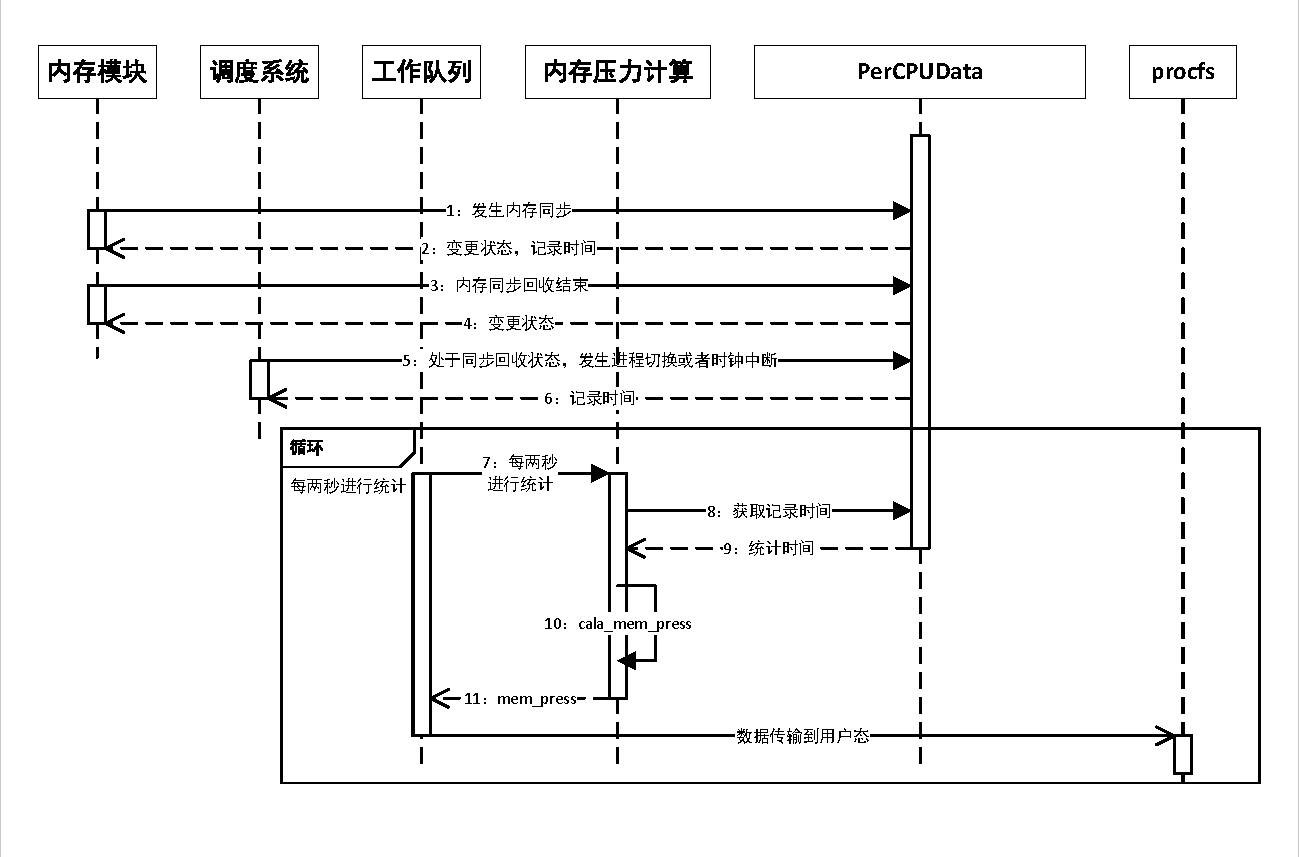
\includegraphics[width=\textwidth, keepaspectratio]{时序图.pdf}
\caption{系统架构时序图}
\label{时序图}
\end{figure}

生产者模块的核心功能是精确捕获内核中与内存回收相关的状态切换时间信息。为实现这一目标,生产者在同步内存回收的起始和结束时刻分别记录时间戳。具体而言,当系统发生直接内存回收时,即进程在分配内存时因内存不足而触发同步回收操作,生产者立即记录起始时间戳,并将该进程的 task\_struct 结构体中的 in\_direct\_reclaim 标志设置为 true,以标识该进程已进入同步回收状态。当同步回收过程结束,进程恢复正常执行时,生产者再次记录结束时间戳,同时将 in\_direct\_reclaim 标志重置为 false。通过计算这两个时间戳的差值,可精确量化本次状态切换所消耗的时间。

此外,为确保全面、准确地捕获所有与状态切换相关的时间消耗,生产者在内核调度过程中进行了额外的时间戳记录。具体实现如下:在每次进程调度发生时(即调用 schedule() 函数时),生产者检查当前即将被调度的进程的 task\_struct->in\_direct\_reclaim 标志。若该标志为 true,表明该进程正处于同步回收状态,即便其即将被调度出去,生产者仍会记录时间戳,以确保其在状态切换上消耗的时间不被遗漏。同时,在每次时钟中断发生时(即 scheduler\_tick() 函数被调用时),生产者检查当前正在运行的进程的 task\_struct->in\_direct\_reclaim 标志。若该标志为 true,表明该进程处于同步回收状态,则记录时间戳,并累加到该 CPU 的每 CPU 变量 direct\_reclaim\_time 中。通过综合同步回收起止事件和内核调度事件的时间戳信息,生产者能够完整地记录所有与状态切换相关的时间消耗。

消费者模块采用工作队列机制实现,其依赖于内核调度器来调度和执行任务。在本系统中,消费者工作队列被配置为每两秒执行一次,其核心任务包括以下四个步骤:


\begin{enumerate}
    \item 数据采集:读取所有 CPU 的 direct\_reclaim\_time 变量的值,这些值代表了在过去两秒内,每个 CPU 上处于同步回收状态的进程所消耗的总时间。
    \item 加权平均计算:将所有 CPU 的同步回收时间进行加权平均,得到整个系统的平均同步回收时间。这一步骤充分考虑了多核系统中各个 CPU 之间的负载均衡情况。
    \item 数据平滑处理:对计算得到的平均同步回收时间应用指数移动平均算法,以消除瞬时波动,准确反映内存压力的长期趋势。
    \item 压力指标计算与输出:根据前文定义的内存压力计算方式,计算得出内存压力值,并通过 procfs 文件系统将其暴露给用户空间,供用户态程序读取和使用。
\end{enumerate}


\subsubsection{工作队列}
我们最终采用了工作队列来进行内存压力的计算。这主要基于以下几个方面的考虑:内存压力的计算上是一个复杂的统计过程,这个过程需要获取互斥锁并进行较长时间的数据处理。这类操作必须在进程上下文中执行,因为它们可能会引起睡眠,不能在中断上下文中完成。此外,内存压力的监控需要周期性执行以跟踪系统状态的变化,这正好契合工作队列提供的延迟执行机制。而且,由于内存压力的计算主要用于系统监控和决策支持,对实时性要求相对不高,可以容忍一定程度的执行延迟。

工作队列作为Linux内核中经过充分验证的标准机制,为异步任务的执行提供了可靠的保障。它能够确保任务在合适的时机得到执行,并在系统负载较高时自动调节执行频率。特别是对于周期性的监控任务,工作队列实现了完善的补偿机制,即使在系统负载较高导致某些统计周期被延迟时,也能通过计算错过的周期数并进行相应补偿,确保监控数据的连续性和准确性。这种机制对于内存压力监控尤为重要,因为它需要准确反映系统在不同时间段的内存使用状况。

如果采用专用内核线程来实现这些功能,不仅需要手动处理线程的创建、销毁和唤醒,还需要考虑各种边界情况,如系统负载过高时的处理策略、错过统计周期的补偿机制等。这些工作不仅增加了代码的复杂度,也提高了出错的可能性。而在内核编程中,边界条件的处理往往是最容易出现问题的地方,这类问题通常难以重现和调试。相比之下,工作队列已经为这些复杂的情况提供了完善的处理机制,使得开发者可以专注于内存压力计算的核心逻辑实现。

从系统资源利用的角度来看,工作队列的共享特性也带来了显著优势。当系统处于空闲状态时,工作队列中的任务会自动停止,避免不必要的资源消耗;当系统负载升高时,工作队列的调度机制能够自动调节任务的执行频率,确保内存压力监控不会对系统性能造成显著影响。这种自适应的特性,结合工作队列成熟的错误处理机制,为内存压力监控提供了一个稳定可靠的执行环境。

\subsubsection{定点数优化}


在实时监控和评估系统内存压力的过程中,频繁的数值计算是不可避免的。特别是在计算内存压力指标以及进行 EMA 平滑处理时,会涉及到大量的浮点数运算。虽然浮点数能够提供较高的数值精度,但在我们关注的内存压力评估场景中,对计算精度的要求并非绝对的,过高的精度反而可能导致不必要的计算资源浪费。因此,我们引入定点数表示法,旨在保证足够精度的前提下,显著提升计算效率。定点数的核心思想在于,通过一个预先确定的缩放因子将实数映射为整数进行存储和运算,从而避免浮点运算。与浮点数动态调整小数点位置不同,定点数的小数点位置是固定的。对于任意实数 \(R\),其定点数表示 \(D\) 可以定义为:

\[
D = \lfloor R \times F \rfloor
\]

其中,\(F\) 表示缩放因子,\(\lfloor \cdot \rfloor\) 表示向下取整操作。为了能够利用计算机底层高效的位移操作来实现乘除运算,缩放因子 \(F\) 通常选择 2 的整数次幂形式,即 \(F = 2^n\)。在本文的应用场景中,我们选择 \(F = 2^{10} = 1024\) 作为缩放因子。这一选择在计算精度和效率之间取得了较好的平衡。

对于任意实数 \(R\), 其定点数表示 \(D\) 会引入量化误差. 量化误差定义为实数与其定点数表示之间的差值:
\[
\epsilon = R - \frac{D}{2^{10}}
\]
由于 \(D\) 是 \(R \times 2^{10}\) 的向下取整结果, 因此存在一个非负实数 \(\delta\)(且 \(\delta < 1\)), 使得:
\[
R \times 2^{10} = D + \delta
\]
将上式两边同时除以 \(2^{10}\), 得到:
\[
R = \frac{D}{2^{10}} + \frac{\delta}{2^{10}}
\]
将此表达式代入量化误差的定义式, 得到:
\[
\epsilon = \frac{\delta}{2^{10}}
\]
由于 \(0 \leq \delta < 1\), 因此量化误差 \(\epsilon\) 满足:
\[
0 \leq \epsilon < 2^{-10} \approx 0.000977
\]
选择\(2^{10}\)作为缩放因子,定点数表示的量化步长为\(2^{-10} \approx 0.000977\)。这意味着对于任意值\(v\),其定点数表示的:最大绝对误差:\(< 0.000977\); 相对误差:\(< 0.000977/v\)。

在定点数的运算过程中,除了量化误差外,还会引入运算误差。假设有两个实数 \(R_1\) 和 \(R_2\), 它们对应的定点数表示分别为 \(D_1\) 和 \(D_2\). 进行加法(或减法)运算时,实际计算的是定点数的和(或差),然后再将结果转换回实数域:
\[
(R_1 \pm R_2) - \frac{D_1 \pm D_2}{2^{10}}
\]
由于\(D_1\)和\(D_2\)的计算都存在误差,且\(0 \leq \epsilon < 2^{-10} \approx 0.000977\),所以
\[
|(R_1 \pm R_2) - \frac{D_1 \pm D_2}{2^{10}}| < 2 \times 2^{-10}
\]

对于两个实数的乘法 \(R_1 \times R_2\), 在定点数运算中, 我们首先计算两个定点数的乘积 \(D_1 \times D_2\), 然后为了保持正确的缩放, 需要将结果右移 10 位(相当于除以 \(2^{10}\)):
\[
(D_1 \times D_2) >> 10
\]
这一操作可以等效为:
\[
(D_1 \times D_2) >> 10 = (R_1 \times R_2) \times 2^{10} + \epsilon_{mul}
\]
其中乘法误差 \(|\epsilon_{mul}| < 2^{-9} + R_1\epsilon_2 + R_2\epsilon_1\)。

在内存压力计算的具体应用中,我们可以采用定点数来替代浮点数进行运算。以 EMA 平滑为例,原始的浮点数计算公式为:
\[
EMA_{new} = EMA_{old} \times \alpha + P_{current} \times (1 - \alpha)
\]

将其转换为定点数形式:
\[
EMA_{new\_fixed} = (EMA_{old\_fixed} \times \alpha_{fixed} + P_{current\_fixed} \times (F - \alpha_{fixed})) >> 10
\]

其中,\(EMA_{old\_fixed}\)、\(P_{current\_fixed}\) 和 \(\alpha_{fixed}\) 分别是 \(EMA_{old}\)、\(P_{current}\) 和 \(\alpha\) 的定点数表示(即乘以 1024 并向下取整的结果)。通过这种转换,我们将原本的浮点数乘法和加法运算替换为整数乘法、加法和位移运算,在保证足够精度的前提下,显著提高了计算速度。

\subsubsection{统计计算}

本节主要是一些工程化一些,主要介绍如何将上述算法落地,防止溢出回绕。

通过 cpu\_clock(cpu) 函数获取 CPU 的时间戳,该函数返回一个 64 位无符号整数(u64),表示从系统启动开始的纳秒级时间计数。当需要计算时间差时,系统使用 32 位无符号整数(u32)来存储差值。这种设计基于以下原理:CPU 时钟是单调递增的,且在较短的测量间隔内(通常是调度周期级别),即使发生了 64 位时间戳的回绕,32 位差值的计算仍然是准确的。这是因为无符号整数的减法运算具有自动处理回绕的特性,当执行 now - start 的操作时,即使 now 小于 start(由于时钟回绕),减法运算仍然能得到正确的时间差。

在底层的时间记录中,32 位无符号整数可以安全地记录约 4.29 秒内的时间差。我们在选择在每次时钟中断的时候进行检查,如果现在正在处理同步中断中,那么我们就需要进行进行记录,4.29秒的时间足够,我们不需要担心溢出。

\begin{algorithm}[H]
    \KwData{group: Memory pressure group structure}
    \KwResult{Updated memory pressure statistics}
    
    % 初始化
    \(deltas[NR\_MEM\_STATES - 1] \gets 0\)\;
    \(nonidle\_total \gets 0\)\;
    Lock(group.stat\_lock)\;
    
    Phase 1: Collect per-CPU data
    \For{each CPU \(cpu\)}{
        \(times[NR\_MEM\_STATES] \gets\) get\_recent\_times(group, cpu)\;
        \(nonidle \gets\) nsecs\_to\_jiffies(times[MEM\_NONIDLE])\;
        \(nonidle\_total \gets nonidle\_total + nonidle\)\;
        
        \For{\(s \gets 0\) to \(MEM\_NONIDLE\)}{
            \(deltas[s] \gets deltas[s] + times[s] \times nonidle\)\;
        }
    }
    
    Phase 2: Update total memory pressure statistics
    \For{\(s \gets 0\) to \(NR\_MEM\_STATES - 2\)}{
        \(group.total[s] \gets group.total[s] + \frac{deltas[s]}{max(nonidle\_total, 1)}\)\;
    }
    
    Unlock(group.stat\_lock)\;
    \Return \(nonidle\_total\)\;
    
    \caption{Memory Pressure Statistics Update}
\end{algorithm}



\subsection{内存压力信息的用户态暴露机制}

\section{最小工作集自适应调整流程}

\subsection{用户态与内核态的交互流程}

\subsection{工作集大小的动态调整策略}

\section{本章小结}